
\chapter{Perspectives\label{chpt:perspectives}}

The work is never perfect, a great deal of unfinished work and theories
linked to this thesis is presented here. 

\section{Reduce memory use in MDFT}

The total CPU time to implement a MDFT minimization using \texttt{\textbf{convolution}}
algorithms is typically 1 to 30 minutes according to the resolution
of grid. But the memory consumed for such a process is typically 1
to 20 G of RAM. This is mainly due to the minimizer L-BFGS-B, which
firstly needs to store several steps of information during the iterations,
and secondly it is in double precision, it is to say that the density
variable $\rho(\mathbf{r},\mathbf{\Omega})$ and the gradient also
need to be stored in double precision, if not, as tested, it leads
to a divergence of result. In addition, during the evaluation of functional,
memory at most 3 times of $\rho(\mathbf{r},\mathbf{\Omega})$ needs
to be stored simultaneously.

There are to ways to get over this memory limit, and both of them
need to modify the L-BFGS-B minimizer, which is a ``blackbox'',
in Fortran 77. 

The simplest way is to change the double precision to float number
of the L-BFGS-B minimizer, this action can reduce the memory needed
by 2. 

And another way to completely pass this limit, is to parallelize is
code to several nodes using MPI. This requires only to modify the
\acs{FFT} and L-BFGS-B process, where their is a mixing of variables
$\rho(\mathbf{r},\mathbf{\Omega})$.

\section{Site-site grid}

The \acs{IET} uses intermolecular spherical coordinates, and cannot
describe huge molecules. \acs{MDFT} uses a homogeneous spatial grid,
thus have the same resolution near and far from the solute. The defeat
of \acs{MDFT} is that for very polar solutes, the grid needed should
be very fine to meet a satisfying result, and in 3D it is a very huge
number, as it treats the same resolution from near to far from the
solute. Another natural way to think about construction of the grid
is like in \ref{fig:Site-site-grid-model}, an spherical grid at each
site of solute. 

\textcolor{red}{(This part needs more brain)}

\begin{figure}[h]
\begin{centering}
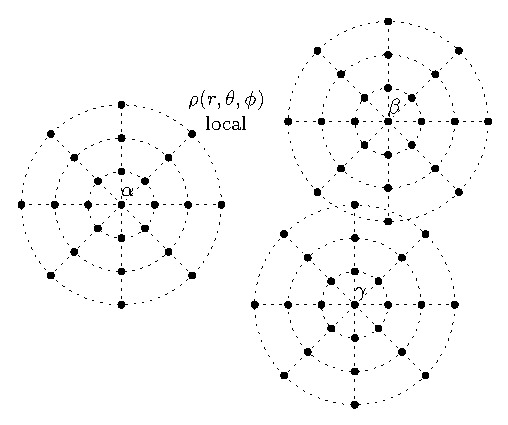
\includegraphics{_figure/site-site}
\par\end{centering}
\caption{Site-site grid model\label{fig:Site-site-grid-model}}
\end{figure}

The idea can be roughly understand as an interaction site treatment
of the solute, with a molecular treatment of the solvent. It is a
matrix of $h_{\text{MS}}(1,2)$ with a full molecular description
of $c_{\text{SS}}(1,2)$. As in \acs{MDFT} the solvent density can
be else than particle-particle distribution functions, it is possible
to have different descriptions for solute and solvent. The formalism
is possible, also as the e\acs{DFT} shares some formalism with c\acs{DFT},
a site description of solute which is used as default in \acs{QM}
calculations should also gives some inspiration to the liquid theory.
(Or I think it is like 3D-RISM, but their is no correspondent \acs{DFT}
theory, nor basis set description of site.) If the sites are expanded
onto spherical harmonics $Y_{lm}$, there is also a rotational invariance
between the sites, and the inhomogeneous angular grid can be thus
ignored, it is only an issue of $\mathbf{r}_{\text{M}}-\mathbf{r}_{\text{N}}$
between site M and N. This is only an idea, the mathematical deduction
is not yet fully verified.

The generalized \acs{OZ} equation to $n$ components
\begin{equation}
h_{\nu\mu}(1,2)=c_{\nu\mu}(1,2)+\rho\sum_{\lambda}x_{\lambda}\int c_{\nu\lambda}(2,3)h_{\lambda\mu}(1,3)\mathrm{d}3
\end{equation}
thus
\begin{equation}
h_{\text{MS}}(1,2)=c_{\text{MS}}(1,2)+\rho\int c_{\text{SS}}(2,3)h_{\text{MS}}(1,3)\mathrm{d}3
\end{equation}
\begin{equation}
h_{\text{NS}}(1,2)=c_{\text{NS}}(1,2)+\rho\int c_{\text{SS}}(2,3)h_{\text{NS}}(1,3)\mathrm{d}3
\end{equation}
Look that $c_{\text{SS}}(2,3)$ is just the bulk \acs{DCF}. The link
between $h_{\text{MS}}(1,2)$ and $h_{\text{NS}}(1,2)$ is a translation
of center $\mathbf{r}_{\text{M}}-\mathbf{r}_{\text{N}}$\textcolor{red}{(?)}.
Therefore, ...

\section{Theories out from the HRF approximation part}

In terms of $\mathcal{F}_{\mathrm{exc}}$, there can be still development
out of HRF approximation, such as 3-body correction.

Apart from the $\mathcal{F}_{\mathrm{exc}}$ term, there are still
many field of study to develop \acs{MDFT}. For example, the evaluation
of external potential $V_{\mathrm{ext}}$, which poses problems of
convergency for molecular solutes, still needs to improve. Note that
this part can be also a functional of solvent density, in this case,
the solute is polarizable, and the $V_{\mathrm{ext}}$ varies during
the minimization. The polarization can be introduced by for example
an extra dipole on the solute.

\section{MDFT Viewer}

This thesis contains originally a segment on visualization. Due to
time limit, it is removed. Viewer is an important part of code development,
which provides beautiful visualization and easy analysis, and helps
to popularize the code. GaussViewer is a good example.

\section{Application to real biological systems, and entropy}

From this thesis we can see that \acs{MDFT} is capable to deal with
some small chemical system, but it is still far from satisfied for
common usage in the domain of bio-chemistry as a complement of \acs{QM}.
For example, for real applications, enthalpy and entropy are also
important, as discussed in ref \citep{Mn-oxo}. The results of \citep{Mn-oxo}
cannot be repeated with \acs{QM} calculations using simply continuum
model as solvent corrections (research subject of my university diploma),
which gives identical tendency of entropy with respect to temperature
(in DMSO). In \acs{MDFT}, the $\mathcal{F}_{\mathrm{id}}$term gives
entropy of information. It is not exactly the same as total entropy
as there are also contribution from charge distribution, etc.
